\section{Enterprise integration patterns and Camel}

\begin{definition}[Integration]
Integration is the art of making different programms (like a database, a website and a desktop-client) work well together. 
\end{definition}

Camel is easily set up with maven: 

\begin{lstlisting}[language=xml]
<project 
xmlns="http://maven.apache.org/POM/4.0.0" 
xmlns:xsi="http://www.w3.org/2001/XMLSchema-instance" 
xsi:schemaLocation="http://maven.apache.org/POM/4.0.0 http://maven.apache.org/xsd/maven-4.0.0.xsd">

  <modelVersion>4.0.0</modelVersion>
  <groupId>org.langbein.michael</groupId>
  <artifactId>RiderAutoParts</artifactId>
  <version>0.0.1-SNAPSHOT</version>
	

	<dependencies>
		<dependency>
			<groupId>org.apache.camel</groupId>
			<artifactId>camel-core</artifactId>
			<version>2.19.2</version>
		</dependency>
		<dependency>
			<groupId>org.slf4j</groupId>
			<artifactId>slf4j-simple</artifactId>
			<version>1.7.25</version>
		</dependency>
	</dependencies>
	
		
	<packaging>jar</packaging>
	
	<build>
		<plugins>
		
			<plugin>
			    <!-- this is for being able to run camel with camel:run -->
				<groupId>org.apache.camel</groupId>
				<artifactId>camel-maven-plugin</artifactId>
				<!-- optional, default value: org.apache.camel.spring.Main -->
				<configuration>
					<mainClass>main.AppMain</mainClass>
				</configuration>
			</plugin>

			<!-- download source code in Eclipse, best practice -->
			<plugin>
				<groupId>org.apache.maven.plugins</groupId>
				<artifactId>maven-eclipse-plugin</artifactId>
				<version>2.9</version>
				<configuration>
					<downloadSources>true</downloadSources>
					<downloadJavadocs>false</downloadJavadocs>
				</configuration>
			</plugin>

			<!-- Set a JDK compiler level -->
			<plugin>
				<groupId>org.apache.maven.plugins</groupId>
				<artifactId>maven-compiler-plugin</artifactId>
				<version>2.3.2</version>
				<configuration>
					<source>${jdk.version}</source>
					<target>${jdk.version}</target>
				</configuration>
			</plugin>

			<!-- Make this jar executable -->
			<plugin>
				<groupId>org.apache.maven.plugins</groupId>
				<artifactId>maven-jar-plugin</artifactId>
				<configuration>
				  <archive>
					<manifest>
						<!-- Jar file entry point -->
						<mainClass>main.AppMain</mainClass>
					</manifest>
				  </archive>
				</configuration>
			</plugin>

		</plugins>
	</build>
</project>
\end{lstlisting}

After the usual maven setup, a simple camel project might look a little something like this: 

\begin{lstlisting}[language=java]
public class AppMain {

	public static void main(String[] args) {
		CamelApp ca = new CamelApp();
		try {
			FtpRoute fr = new FtpRoute();
			ca.init(fr);
			ca.run();
		} catch (Exception e) {
			e.printStackTrace();
		}
	}
}
\end{lstlisting}

\begin{lstlisting}[language=java]
public class CamelApp {
	private CamelContext cc;
	public CamelApp () {
		cc = new DefaultCamelContext();
	}
	public void init (RouteBuilder rb) throws Exception {
		cc.addRoutes(rb);
	}
	public void run() throws Exception {
		cc.start();
        Thread.sleep(10000);
        cc.stop();
	}
}
\end{lstlisting}

\begin{lstlisting}[language=java]
public class FtpIncomming extends RouteBuilder{
	public void configure() throws Exception {
		RouteDefinition rd;
		rd = from("file:inbox/?noop=true");
		rd = rd.process(new BodyLogger());
		rd = rd.to("file:outbox/?fileName=out.txt");
	}
}
\end{lstlisting}
\begin{lstlisting}[language=java]
public class BodyLogger implements Processor{
	public void process(Exchange ex) throws Exception {
		String body = ex.getIn().getBody().toString();
		System.out.println("Der Body ist: " + body);
	}
}
\end{lstlisting}

Here, $file:data/inbox?noop=true$\footnote{ It is not well documented how a path in the file-component should be specified. The answer is: absolute paths (on windows and linux alike): 
\inlinecode{"file://C:/Users/Langbein_M/Desktop/java_ee_workspace/mycam/src/main/resources/gkd_testdatensatz?fileName=iw_mn.csv&noop=true"}
Relative paths: 
\inlinecode{"file:src/main/resources/in?noop=true"}} is the first endpoint, created from the FileComponent. from returns a FileProducer
Here, from takes a string instucting it to access the FileComponent, and instruct it to create a file-endpoint and a FileProducer. The FileProducer sends a message containing the file to filter.  


\subsection{Basic data-structures: exchange and message}
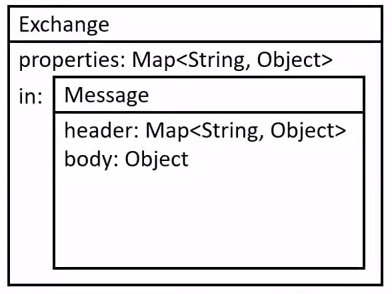
\includegraphics[width=0.3\textwidth]{images/exchange.png}

Properties are for camel-internal use only, whereas headers contain information that other endpoints might find useful. 

\subsection{Text processing}

For all marshaling libraries that java offers, camel has a component. 

\begin{lstlisting}[language=java]
package de.bayern.lfu.gimp.routes.simple;

import javax.xml.bind.JAXBContext;

import org.apache.camel.builder.RouteBuilder;
import org.apache.camel.converter.jaxb.JaxbDataFormat;
import org.apache.camel.dataformat.bindy.csv.BindyCsvDataFormat;
import org.apache.camel.model.dataformat.JsonLibrary;
import org.springframework.stereotype.Component;

@Component
public class SimpleRoutes extends RouteBuilder{

	@Override
	public void configure() throws Exception {
		// This is a simple route that reads csv from in, 
		// converts it to json and delivers it to out. 
		
		BindyCsvDataFormat csvFormat = new BindyCsvDataFormat(People.class);
		
		from("file:src/main/resources/in?noop=true")
		.id("someSimpleRoute")
		.log("Vor Konversion: ${body}")
		.unmarshal(csvFormat)
		.marshal().json(JsonLibrary.Jackson)
		.log("Nach Konversion: ${body}")
		.to("file:src/main/resources/out");
	}

}
\end{lstlisting}

\begin{lstlisting}[language=java]
package de.bayern.lfu.gimp.routes.simple;

import org.apache.camel.dataformat.bindy.annotation.CsvRecord;
import org.apache.camel.dataformat.bindy.annotation.DataField;

@CsvRecord( separator = ";", skipFirstLine = true, generateHeaderColumns = true )
public class People {

	@DataField(pos = 1)
	private String FirstName;
	@DataField(pos = 2)
	private String LastName;
	@DataField(pos = 3)
	private int IQ;
	@DataField(pos = 4)
	private String Occupation;
	
	public String getFirstName() {
		return FirstName;
	}
	public void setFirstName(String firstName) {
		FirstName = firstName;
	}
	public String getLastName() {
		return LastName;
	}
	public void setLastName(String lastName) {
		LastName = lastName;
	}
	public int getIQ() {
		return IQ;
	}
	public void setIQ(int iQ) {
		IQ = iQ;
	}
	public String getOccupation() {
		return Occupation;
	}
	public void setOccupation(String occupation) {
		Occupation = occupation;
	}
	
}
\end{lstlisting}

\subsection{Routing based on predicates}
Predicates are expressions that return a boolean\footnote{This makes predicates a subset of anonymous functions.}, usually written in one of camels scripting languages. 
Commonly used scripting languages are \emph{simple} for quickly accessing headers, or xpath for reading information from xml-files. You can even combine multiple language-expression into one by using the \inlinecode{PredicateBuilder}.

\begin{lstlisting}[language=java]
BindyCsvDataFormat messnetz = new BindyCsvDataFormat(Messnetz.class);
Predicate isMessnetz = simple("${in.header.CamelFileName} equals 'iw_mn.txt'");

from("ftp://{{username}}@{{hostname}}:{{port}}/{{dirname}}")  // <-- hole von ftp
	.id("GrundwasserChemieFtpRoute")
	.choice()
		.when(isMessnetz)					// <-- welche Art von Tabelle?
			.unmarshal(messnetz)            // <-- entpacken zu pojos
			.split(body())                  // <-- aufteilen in indiv. reihen
			.to("hibernate");               // <-- in db
\end{lstlisting}




\subsection{Processors versus beans}
You can use a processor in a route with \inlinecode{.process(myProcessorInstance)}, whereas you would use a bean in a route with \inlinecode{.beanRef("nameOfMyBean", "methodToCall")}. What's the difference between the two?
\begin{itemize}
    \item A processor  needs to implement \inlinecode{Processor}, which is camel-specific. A bean on the other hand does not need to know it's beeing used in camel. 
    \item A processor is usually intantiated by you inside the route-definition, whereas beans are instantiated by the camel/spring-context. Beans therefore need to be either created in some spring-config-file or annoted with \inlinecode{@component}.
    \item A processor is only allowed to use one method, the \inlinecode{process(Exchange exchange)} method. Beans, however, may expose multiple methods\footnote{However, those methods should ideally only accept one parameter. Camel by default passes a bean-method the body of the exchange. To do so, camel tries its best to convert the body-type to whatever type the bean expects. If you really need more than one parameter, you'll have to use camel-specific annotations to explain to camel what to pass into that method.}. 
\end{itemize}

\subsection{Camel SQL component}

You can fetch data from the database and write data into it. 
But there is one catch: jdbc cannot be the first element in your chain - it must'nt be in the from statement. 
The reason is, that it needs a command to get startet consuming. So from would first produce a command, which would be routed to the jdbc component, who's response would go further down the route. 

\subsection{Configuring camel}

\paragraph{Gonfiguring global variables in a *.properties file} Just like spring, you can configure camel using a *.properties file. 

\begin{lstlisting}[language=java]
PropertiesComponent prop = context.getComponent("properties", PropertiesComponent.class);
prop.setLocation("classpath:gimp.properties");
\end{lstlisting}

After letting camel know where to look for properties, they can be parsed into into urls like this: \inlinecode{"file:\{\{location\}\}?noop=true"}, or be extracted into variables like this: \inlinecode{String inboxDir = context.resolvePropertyPlaceholders("\{\{file.inbox\}\}");}.


\paragraph{Registering beans in the camel-registry} Sometimes you also will have to add beans to the camel-registry. For example, the jdbc-component requires you to have registered a datasource before you call it in any route. Unfortunately, camel does not expose an api to add beans to the camel-registry\footnote{The reason is that camel can use different registries. It is possible to add beans to an instance of \inlinecode{SimpleRegistry} by using \inlinecode{put} and to a \inlinecode{JndiContext} by using \inlinecode{bind}, but not to add one to an instance of \inlinecode{ApplicationContextRegistry}.}. Instead, you need to keep a reference to the registry when you create the camel-context.

\begin{lstlisting}[language=java]
this.camelRegistry = new SimpleRegistry();
this.camelContext = new DefaultCamelContext(this.camelRegistry);

...

this.camelRegistry.put("SomeSimpleBean", new MyBean());
\end{lstlisting}

There is an alternative approach, however. When camel is used inside a spring-context (which it almost always is), it will always use an instance of \inlinecode{ApplicationContextRegisty}. That means that any \inlinecode{@Bean} that is defined in any \inlinecode{@Configuration} class will be available in a camel-uri.


\subsection{Writing custom components}

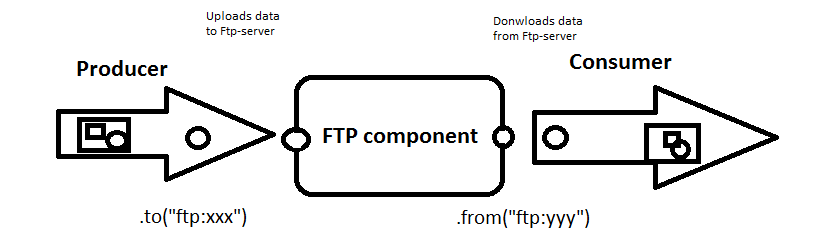
\includegraphics[width=11cm]{images/camel.png}

To understand better how camel works, it is instructive to create a custom component.

Consumers have the job of taking raw datafiles form an external system and wrapping them in an exchange. 
Producers have the job of taking an exchange containing data, processing the data then pass the data to an external system. 
Note that producers extend processors. 

For example, in the ftp-component: 
The consumer takes files from the ftp-server and then wraps them in an exchange. It then tells a (yet to be specified by the routebuilder) producer from another component to process the exchange. 
The fpt-processor on the other hand will be passed to some (yet to be specified by the routebuilder) consumer to receive an exchange containing the data and then send the data to the ftp-server.

\begin{itemize}
    \item Raw data is fed into the consumer of component a (from ftp-server into ftp-server-component-consumer). 
    \item The consumer wraps the raw data into an exchange.
    \item The camel context supplies the producer of component b (could be anything, here we'll assume a jms-component) to the consumer of component a.
    \item The consumer of component a tells the producer of component b to process the exchange. 
    \item The producer does so and then sends the processed data to component b (from jms-component-producer to jms-que).
\end{itemize}

As you can see, there is always just one from and one to. 
The routebuilder can however do some routing or duplicate messages to send them to multiple targets. Then, it would send producers form (say) a ftp-component and a jms-component to the consumer of a filesystem-component, to have a file be sent to both an ftp-server and a jms-que.


So when would I write a custom component instead of a custom processor?
You write a custom processor when you need to make changes to a targets data - e.g. the file. You would for example need a processor to read out information from a zrxp-file. You would write a component, when the datas source or target is entirely new - like github, a sftp-server, google-maps-api, outlook-smtp, a spark-cluster, etc. 

\begin{lstlisting}[language=java]
public class MyComponentTest extends CamelTestSupport {

    public void testTimerInvokesBeanMethod() throws Exception {
        MockEndpoint mock = getMockEndpoint("mock:result");
        mock.expectedMinimumMessageCount(1);       
        
        assertMockEndpointsSatisfied();
    }

    protected RouteBuilder createRouteBuilder() throws Exception {
        return new RouteBuilder() {
            public void configure() {
                from("mycomponent://foo")    // will send a message every 500ms
                  .to("mycomponent://bar")   // prints message to stdout
                  .to("mock:result");       // to actually test that a message arrives
            }
        };
    }
}
\end{lstlisting}

\begin{lstlisting}[language=java]
public class MyComponent extends DefaultComponent {

    protected Endpoint createEndpoint(String uri, String remaining, Map<String, Object> parameters) throws Exception {
        Endpoint endpoint = new MyEndpoint(uri, this);
        setProperties(endpoint, parameters);
        return endpoint;
    }
}
\end{lstlisting}

\begin{lstlisting}[language=java]
public class MyEndpoint extends DefaultEndpoint {

    public MyEndpoint() {
    }

    public MyEndpoint(String uri, MyComponent component) {
        super(uri, component);
    }

    public Producer createProducer() throws Exception {
        return new MyProducer(this);
    }

    public Consumer createConsumer(Processor processor) throws Exception {
        return new MyConsumer(this, processor);
    }

    public boolean isSingleton() {
        return true;
    }
}
\end{lstlisting}

\begin{lstlisting}[language=java]
public class MyConsumer extends ScheduledPollConsumer {
    private final MyEndpoint endpoint;

    public MyConsumer(MyEndpoint endpoint, Processor processor) {
        super(endpoint, processor);
        this.endpoint = endpoint;
    }

    // poll method will fire every 500 ms by default 
    protected int poll() throws Exception {
        Exchange exchange = endpoint.createExchange();

        // create a message body
        Date now = new Date();
        exchange.getIn().setBody("Hello World! The time is " + now);

        try {
            // send message to next processor in the route
            getProcessor().process(exchange);
        } finally {
            // log exception if an exception occurred and was not handled
            if (exchange.getException() != null) {
                getExceptionHandler().handleException("Error processing exchange", exchange, exchange.getException());
            }
        }

        // we consumed 1 message
        return 1;
    }

}
\end{lstlisting}

\begin{lstlisting}[language=java]
public class MyProducer extends DefaultProducer {
    private static final transient Logger LOG = LoggerFactory.getLogger(MyProducer.class);
    private MyEndpoint endpoint;

    public MyProducer(MyEndpoint endpoint) {
        super(endpoint);
        this.endpoint = endpoint;
    }

    public void process(Exchange exchange) throws Exception {
    	LOG.info(exchange.getIn().getBody().toString());
        System.out.println(exchange.getIn().getBody());    
    }

}
\end{lstlisting}

\subsection{Writing custom data-types}

Very often, the processing we want to do consists only of reading out a specific filetype. 
Usually, we'd implement a processor, but we can be more specific yet. We can implement a custom filetype and use it in the methods $masrhal$ (convert X to the filetype) and $unmarshal$ (put content of filetype in exchange).

\begin{lstlisting}[language=java]
public void configure() throws Exception {
    from("file://C:/in/?fileName=MyFile.txt&noop=true")
    .marshal(new PdfTextDataFormat())
    .to("file://C:/out/?fileName=MyFile.pdf");
}
\end{lstlisting}

\begin{lstlisting}[language=java]
public PdfTextDataFormat implements DataFormat {

    /**
    * from object ( in this case, to String ) to stream
    */
    public void marshal(Exchange exchange, Object graph, OutputStream stream) {
        // Don't do this: String s = (String) o;
        // Instead, use Camel type converters like this:
        String s = exchange.getContext().getTypeConverter().mandatoryConvertTo(String.class, graph);
        // Create a PDF document from the string and convert it into a byte array
        byte[] bytes = ...;
        IOUtils.write(bytes, stream);
        // Don't close output stream here
    }
    
    /**
    * from stream to object ( in this case, to String )
    */
    public Object unmarshal(Exchange exchange, InputStream stream) throws Exception {
        byte[] bytes = IOUtils.toByteArray(stream);
        // Use a tool like PDFBox to create text from your bytes.
        String text = ...;
        // If we want, we can set the unmarshalled text back into the exchange's out message
        Message out = exchange.getOut();
        out.setBody(text);
        // Don't close input stream here
        return text;
    }
}
\end{lstlisting}

\subsection{Gluing routes together}

With the \inlinecode{direct}  component. 

\subsection{Mocking an input}

Principally, camel assumes that the input to a route comes from somewhere outside. However, we can mock that outside from within the application using the producer-template.

We let the route start \inlinecode{form("direct:someName")}. 

\begin{lstlisting}[language=java]
from("direct:someName") // <-- wait for context to send a message into direct
.to("file:...");
\end{lstlisting}

And then we put input in it with:

\begin{lstlisting}[language=java]
ProducerTemplate template = ctxt.createProducerTemplate();
template.sendBody("direct:someName", "This is a test message");
\end{lstlisting}

\subsection{Manually starting a camel route}

Principally, camel routes are meant to be set up once and only once on startup. There they will remain in the context waiting for content to arrive at the from-end. The camel app is then supposed to be cuontinuously running on the server. However, on some occassions we might only want to set up a route on command.

First, we have to avoid that the route starts by itself. 

\begin{lstlisting}[language=java]
from("file:....")
.routeId("sendMail")
.autoStartup(false)
.setHeader("Subject", constant("camelnachricht"))
.setHeader("To", constant("michael.langbein@lfu.bayern.de"))
.to("smtp://UMWELT\\Langbein_M@relay.rz-sued.bayern.de:25?password=michael86&from=alarmplaene@lfu.bayern.de");
\end{lstlisting}

Then we start the route with:

\begin{lstlisting}[language=java]
ctxt.startRoute("sendMail");
\end{lstlisting}

However, most often this is not the most elegant approach. Usually it is better to let the route be initiated on startup, and then have it listen on some \inlinecode{direct:something} element. Only once you send something into the \inlinecode{direct} the route goes on the enricht the message.

\begin{lstlisting}[language=java]
from("direct:startSignal") // <-- wait for app to send a message into direct
.pollEnrich("file:....") // <-- then fetch something (otherwise, this would have stood under from() )
.setHeader("Subject", constant("camelnachricht"))
.setHeader("To", constant("michael.langbein@lfu.bayern.de"))
.to("smtp://UMWELT\\Langbein_M@relay.rz-sued.bayern.de:25?password=michael86&from=alarmplaene@lfu.bayern.de");
\end{lstlisting}

You trigger the now already running and waiting route to actually fetch something from pollEnrich by sending in a minimal message: 

\begin{lstlisting}[language=java]
camelContext.createProducerTemplate().sendBody("direct:startSignal", "go and fetch something from file!");
\end{lstlisting}

\subsection{Aspect orientation}
You can alter and wrap any part of a camel route by using \inlinecode{adviceWith}.

\subsection{Testing}

There are two basic approaches that you are going to use in testing camel routes. 

The first is testing one specific step in the route. Say you have defined a custom processor and now you want to check that it processes all kinds of inputs correctly. This is acchieved by creating a small testroute, usually consisting of one mock-input, your processor, and finally one mock output. 

The other approach is testing a whole route. You might have defined a really complex route and want to ensure that the stuff that comes out at the end has the right form. Here it doesn't make sense to write a custom route, obviously. Instead, we create some test-input and catch whatever arrives at the output. The test-input is created by sending stuff with \inlinecode{producerTemplate} to the routes \inlinecode{from}. The catching of the output is acchieved by using \inlinecode{adviceWith} to wrap a mock-endpoint around the \inlinecode{to}.\footnote{The single best web-resource on the topic that I could find was http://opensourceconnections.com/blog/2014/04/24/correctly-using-camels-advicewith-in-unit-tests/.}

\subsubsection{Basic setup}

\begin{lstlisting}[language=java]
public class SimpleRoutes extends RouteBuilder{

	@Override
	public void configure() throws Exception {
		// This is a simple route that reads csv from in, 
		// converts it to xml and delivers it to out. 
		
		BindyCsvDataFormat csvFormat = new BindyCsvDataFormat(People.class);
		
		from("file:src/main/resources/in?noop=true")
		.id("someSimpleRoute")
		.log("Vor Konversion: ${body}")
		.unmarshal(csvFormat)
		.marshal().json(JsonLibrary.Jackson)
		.log("Nach Konversion: ${body}")
		.to("file:src/main/resources/out");
	}

}
\end{lstlisting}

The simplest setup for this route could look like this: 

\begin{lstlisting}[language=java]
public class SimpleRoutesTests extends CamelTestSupport {
	
	// Giving the route to the camel context
	@Override
	protected RoutesBuilder createRouteBuilder() throws Exception {
		return new SimpleRoutes();
	}
	
	@Test
	public void testFileConverted() throws Exception {
		String body = "FirstName;LastName;IQ;Occupation\r\n" + 
				"Joe;Dalton;110;bandit\r\n" + 
				"Jack;Dalton;105;bandit\r\n" + 
				"William;Dalton;100;bandit\r\n" + 
				"Averal;Dalton;80;bandit\r\n" + 
				"Luke;Lucky;115;cowboy\r\n";
		
		template.sendBodyAndHeader("file:src/main/resources/in", body, Exchange.FILE_NAME, "testfile.csv");
		Thread.sleep(1000);
		File target = new File("src/main/resources/out/testfile.csv");
		assertTrue("Teste, ob Datei in out angekommen ist.", target.exists());
	}
}
\end{lstlisting}


\subsubsection{Splicing in mocks}

This is an examlple of using advice to splice in a mock-endpoint into an existing route. 

\begin{lstlisting}[language=java]
public class SimpleRoutesTests extends CamelTestSupport {
	
	// Giving the route to the camel context
	@Override
	protected RoutesBuilder createRouteBuilder() throws Exception {
		return new SimpleRoutes();
	}
	
	@Override
	public boolean isUseAdviceWith() {
		// When using this, we need to start camelContext manually.
		// Assures that mocks will already be spliced in right when context starts.
		return true; 
	}
	
	@Before
	public void mockEndpoints() throws Exception {
		AdviceWithRouteBuilder awrb = new AdviceWithRouteBuilder() {
			@Override
			public void configure() throws Exception {
				interceptSendToEndpoint("file:src/main/resources/out")
					//.skipSendToOriginalEndpoint()
					.to("mock:targetDir");
			}
		};
		context.getRouteDefinition("someSimpleRoute").adviceWith(context, awrb);
	}
	
	
	@Test
	public void testFileConverted() throws Exception {
		String body = "FirstName;LastName;IQ;Occupation\r\n" + 
				"Joe;Dalton;110;bandit\r\n" + 
				"Jack;Dalton;105;bandit\r\n" + 
				"William;Dalton;100;bandit\r\n" + 
				"Averal;Dalton;80;bandit\r\n" + 
				"Luke;Lucky;115;cowboy\r\n";
		MockEndpoint targetDir = getMockEndpoint("mock:targetDir");
		targetDir.expectedMessageCount(1);
		
		context.start();
		
		template.sendBodyAndHeader("file:src/main/resources/in", body, Exchange.FILE_NAME, "testfile.csv");
		Thread.sleep(1000);
		
		File target = new File("src/main/resources/out/testfile.csv");
		assertTrue("Teste, ob Datei in out angekommen ist.", target.exists());
		targetDir.assertIsSatisfied();
		
		context.stop();
	}
}
\end{lstlisting}

\subsubsection{Simulating errors}

\subsubsection{Using notifyBuilder and browsableEndpoint}
These two allow you to peak into a running route without having to use aspects.